\documentclass[12pt, a4paper]{article}

\usepackage[utf8]{inputenc}
\usepackage{parskip}
\usepackage[margin=2.5cm]{geometry}
\usepackage[danish]{babel}
\usepackage{lmodern}
\usepackage{booktabs}
\usepackage{float}
\usepackage{pdfpages}
\usepackage[T1]{fontenc}
\usepackage{todonotes}
\usepackage[danish=guillemets]{csquotes}

\title{
  Projektbeskrivelse\\
  {\large eksamensprojekt DDU (teknikfag A)}
}

\author{Jeppe Bøgeskov og Alexander Schade}

\begin{document}

\maketitle

\section*{Valgte projektoplæg}
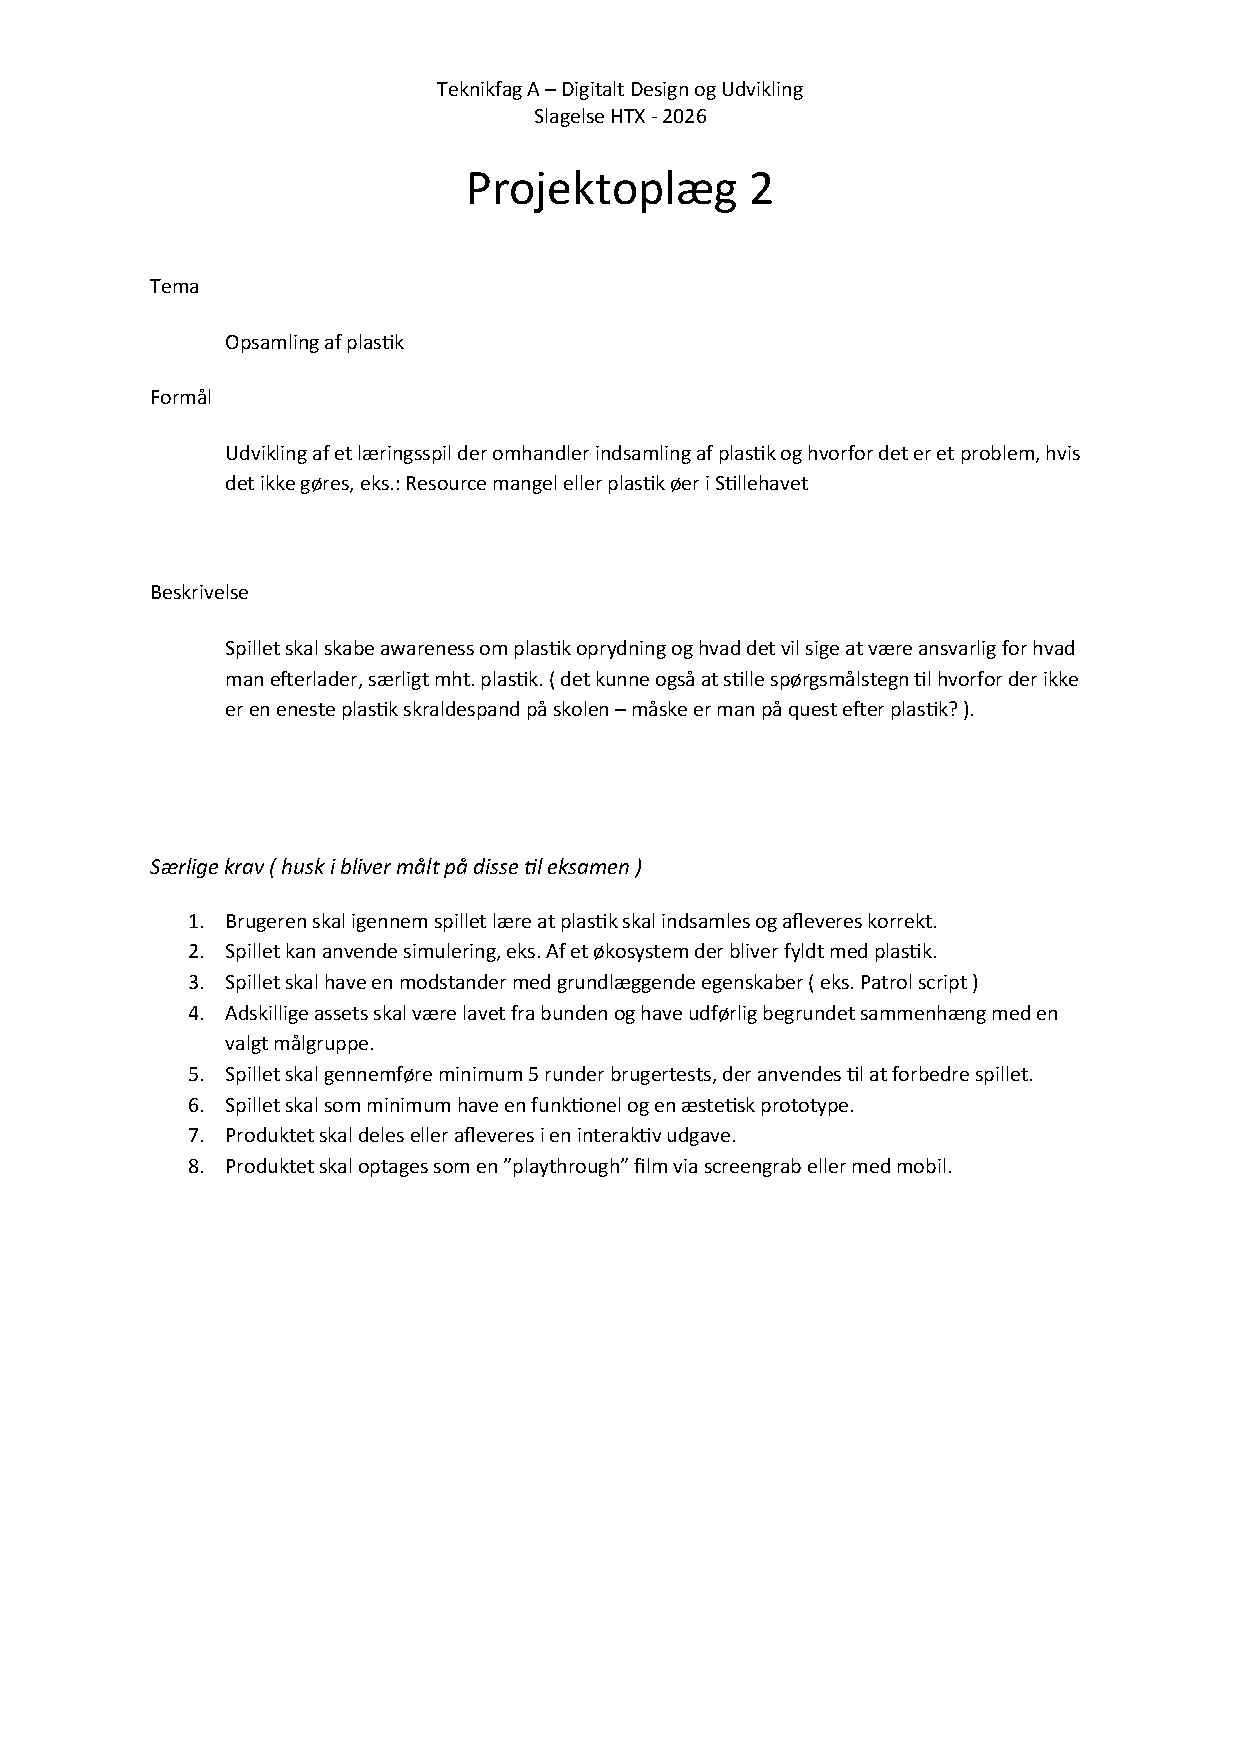
\includepdf[pages=-]{valgte_oplaeg.pdf}

\section*{Problemformulering}
Udkastet til problemformuleringen, der findes interessant er:
\begin{displayquote}
Hvordan kan man lave et spil, hvor havstrømme simuleres og samtidig gøre det interessant for en spiller at navigere i, som har til formål at bringe et moralsk budskab om forurening og \textit{vise} det til spilleren, ikke \textit{fortælle} det, men heller ikke forcere det frem?
\end{displayquote}
\newpage

\section*{Udkast til problemanalyse}
\todo[inline]{Skriv udkast til problemanalyse}
\newpage

\section*{Overvejelser om projektets indhold}
\todo[inline]{Elaborer.}
\newpage

\section*{Tidsplan}
\subsection*{Tid-resurser}
90 moduler a en times varighed.
\subsection*{Vigtige datoer}
\paragraph{Projektstart} mandag d. 9. marts 2026
\paragraph{Frist for godkendelse af projektbeskrivelse} mandag d. 16. marts 2026
\paragraph{Midtvejsdato} mandag d. 13. april 2026
\paragraph{Projektugestart} fredag d. 23. april 2026
\paragraph{Projektugeslut} fredag d. 29. april 2026
\paragraph{Afleveringsfrist for produkt og rapport} torsdag d. 18. maj 2026
\subsection*{Arbejdsuger (sprints)}
\begin{table}[H]
  \centering
  \begin{tabular}{ll}
    \toprule
    Ugenr. & startdag \\
    \midrule 
    11 & mandag d. 9. marts 2026 \\
    12 & mandag d. 16. marts 2026 \\
    13 & mandag d. 23. marts 2026 \\
    14 & mandag d. 30. marts 2026 \\
    15 & mandag d. 6. april 2026 \\
    16 & mandag d. 13. april 2026 \\
    17 & mandag d. 20. april 2026 \\
    18 & mandag d. 27. april 2026 \\
    19 & mandag d. 4. maj 2026 \\
    20 & mandag d. 18. maj 2026 (\textit{\textbf{Obs. afleveringsfrist}}) \\
    \bottomrule
  \end{tabular}\caption{Viser de pågældende uger, hvor projektet er verserende.}
\end{table}
\end{document}
